\documentclass[12pt]{book}
\usepackage[hmargin=0.6in,vmargin=1in]{geometry}
\usepackage{amsmath}
\usepackage{amsthm}
\usepackage[rightcaption]{sidecap}
\usepackage{graphicx}
\usepackage{float}
\usepackage{placeins}
\usepackage{enumerate}
\usepackage{amssymb}
\usepackage{wrapfig}
\usepackage[dvipsnames]{xcolor}
\usepackage{tikz,lipsum,lmodern}
\usepackage[most]{tcolorbox}
\usepackage{hyperref}
\hypersetup{
    colorlinks=true,
    linkcolor=blue,
    filecolor=magenta,
    urlcolor=cyan,
}

\title{Using fancyhdr for Custom Page Header and Footers in a Two-sided Document}

\usepackage{etoolbox}
\makeatletter
% no new page for \chapter
\patchcmd{\chapter}{\if@openright\cleardoublepage\else\clearpage\fi}{}{}{}
% don't change the pagestyle
\patchcmd{\chapter}{\thispagestyle{plain}}{}{}{%
    % example for a warning, 'Package' in text necessary to make TexStudio show it.
    \GenericWarning{(preamble)\@spaces\@spaces\@spaces\@spaces}{Package preamble Warning: patching \string\chapter\space did not work.}}

% allow floats on top of the page with a new chapter
\patchcmd{\chapter}{\global\@topnum\z@}{}{}{}
% if not commented out, first paragraph will be indented
\patchcmd{\chapter}{\@afterindentfalse}{}{}{}
%\makeatother

\usepackage{titlesec}
\titleformat{\chapter}{\normalfont\bfseries\Large}{\thechapter.\quad}{0pt}{}
\titlespacing{\chapter}{0pt}{-5pt}{4pt}% left space, top space, bottom space



\usepackage{fancyhdr}
% Clear off all default fancyhdr headers and footers
\fancyhf{}
\pagestyle{fancy}

\addtolength{\headheight}{\baselineskip}

\fancyhead[L]{\leftmark}
\renewcommand{\chaptermark}[1]{\markboth{\MakeUppercase{#1}}{}}
%\fancyhead[L]{\textbf{\sectiontitle}}
\fancyhead[R]{\sffamily\itshape Lecture Notes on Biophysics}
% Custom text at the left edge of odd pages, and right edge of odd pages.
%\fancyhead[LO,RE]{\sffamily\itshape Fun with fancyhdr}

% Repeat for \fancyfoot if needed, e.g.
% Some decorative symbol at the centre of both odd and even pages
\fancyfoot[L]{\sffamily\itshape Linn Abraham , MGM College of Nursing}
\fancyfoot[C]{\thepage}
\fancyfoot[R]{ September 2020}
% Set this length to 0pt if you don't want any lines!
\renewcommand{\headrulewidth}{2pt}
\pagenumbering{roman}
% Apply the fancy header style
\usepackage{lipsum}
\begin{document}
\setcounter{secnumdepth}{0}

\title{Electricity and Electromagnetism}
\maketitle
\tableofcontents
\newpage

\setcounter{page}{1}
\graphicspath{ {../} }
\chapter{Electricity}
%\subsection{Basics of Electricity}
There are two types of electricity:
\begin{itemize}
	\item static electricity
	\item current electricity
\end{itemize}

\begin{figure}
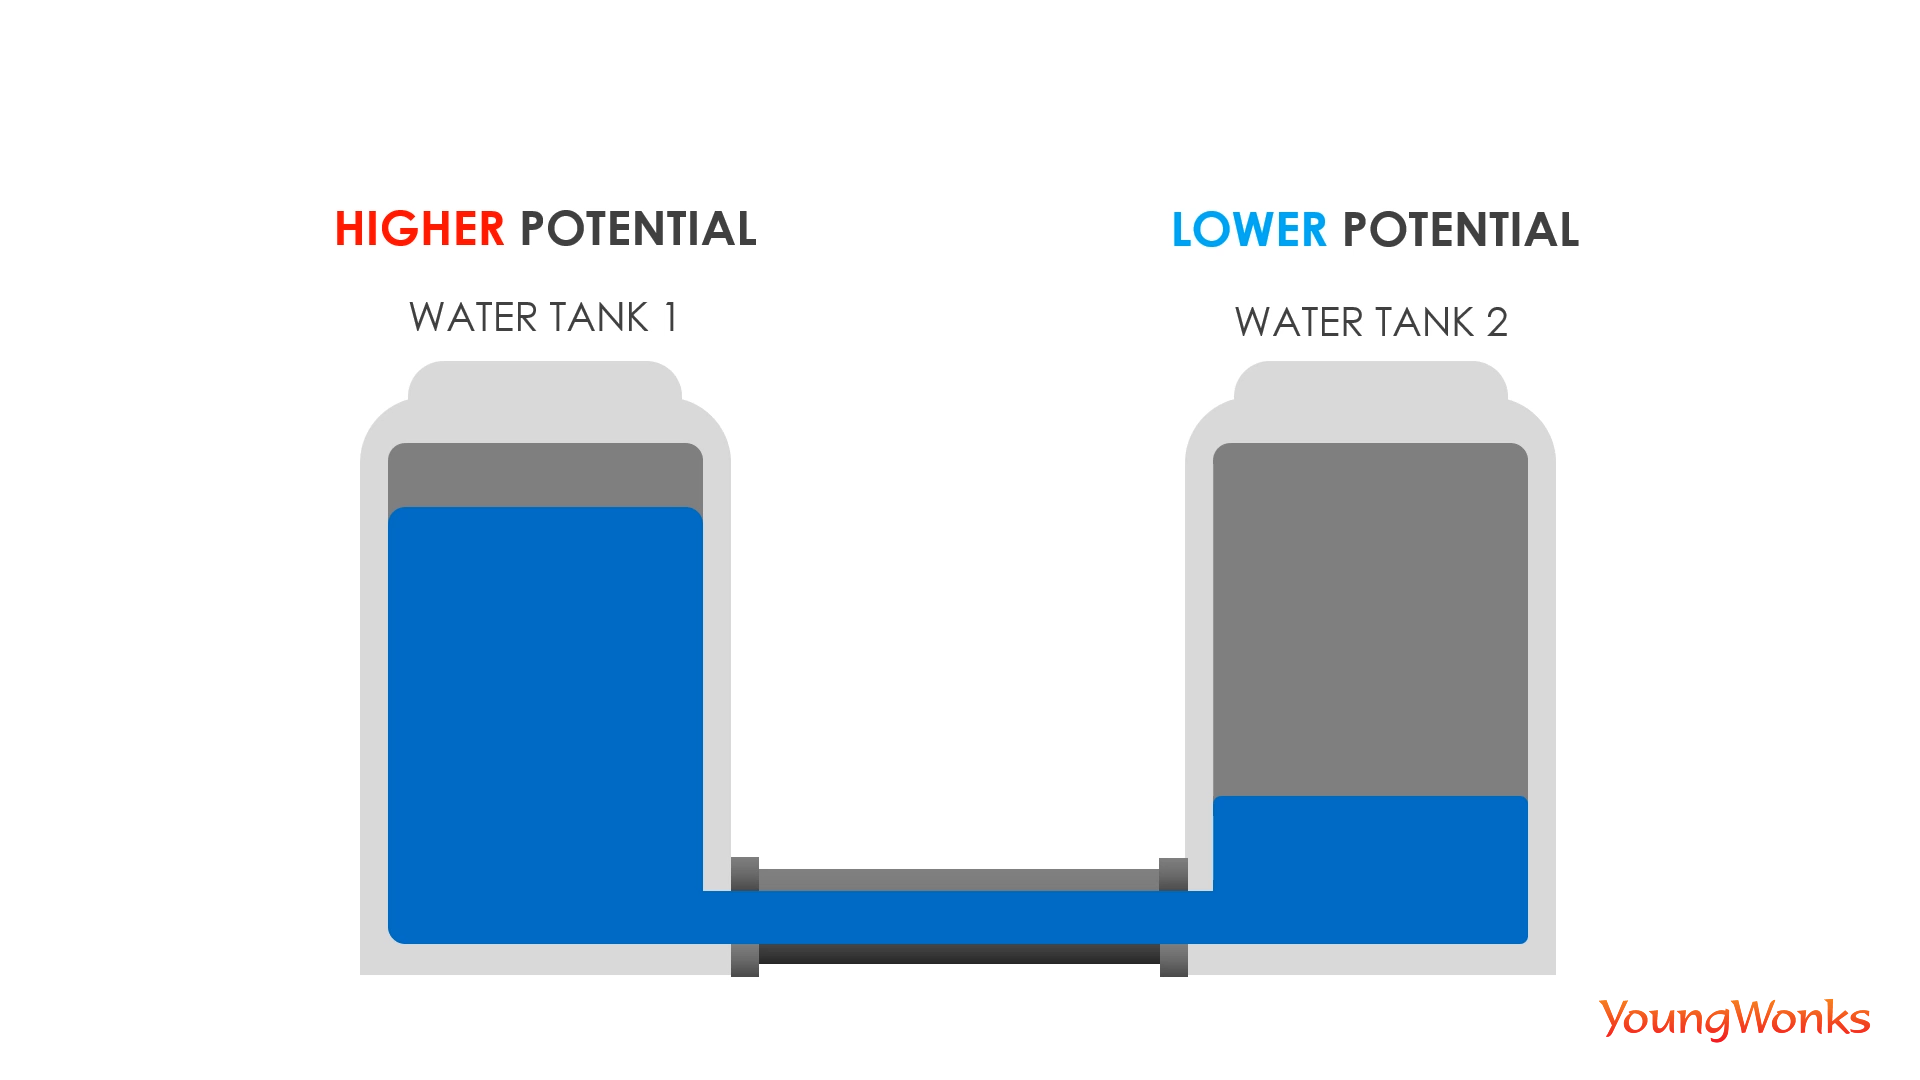
\includegraphics[scale=0.15]{Water_Flow_1.png}

\caption{potential difference}
\end{figure}

\subsection{Voltage}
\begin{itemize}
  		\item Voltage is the potential difference  between two points which is the change in potential energy per charge.  For example, every battery has two terminals, and its voltage is the potential difference between them.
  		 $$ V = \frac{\Delta E}{\Delta q}$$

  		 \item The SI unit is J/C or Volts (V).
  	\item Voltage is not the same as energy. Voltage is the energy per unit charge. Thus a motorcycle battery and a car battery can both have the same voltage , yet one stores much more energy than the other.
\end{itemize}
\subsection{Current}
Electric current measures the rate of flow of charges in a conductor.
$$I = \frac{\Delta Q}{\Delta t} $$

Thus the SI unit of current is C/s or Ampere (A).

\subsection{Resistance}
The opposition to the flow of electric current in an electric circuit is known as resistance. The SI unit of electrical resistance is called Ohm.
\subsection{Ohm's Law}
Ohm's law gives the relation between the relation between voltage and current.
\begin{tcolorbox}[title=Ohm's Law]
%description{

“The current in a conductor is linearly proportional to the difference
of potential between any two points and inversely proportional to the
resistance, provided physical conditions such as temperature, pressure, etc. remain the same.
\end{tcolorbox}

\section{Diagnostic Methods}
\subsection{EEG}


\begin{tcolorbox}[title=Supplementary Information]
Q. How is voltage (potential difference) created across the cell membrane of a neuron in its resting state?

\begin{itemize}
\item The thin cell membrane separates electrically neutral fluids having differing concentrations of ions, the most important varieties being Na+, K+, and Cl-.


\item Free ions will diffuse from a region of high concentration to one of low concentration (diffusion). But the cell membrane is semipermeable.

\item In its resting state, the cell membrane is permeable to K+ and Cl-, and impermeable to Na+.

\item The Coulomb force prevents the ions from diffusing across in their entirety.
\end{itemize}

\end{tcolorbox}
\subsubsection{Basics}

An EEG is a recorded measurement of the voltages appearing at the scalp surface due to the electrical activity of the brain.
\subsubsection{Principle Working and Uses}
Refer to text.

\subsection{ECG}

\subsubsection{Principle}
\begin{itemize}
	\item An electrocardiogram (ECG) is a record of the voltages created by the wave of depolarization and subsequent repolarization in the heart.

	\item Just as nerve impulses are transmitted by depolarization and repolarization of adjacent membrane, the depolarization that causes muscle contraction can also stimulate adjacent muscle cells
	to depolarize (fire) and contract.

	\item Depolarization of the heart muscle causes it to contract. After contraction it is repolarized to ready it for the next beat.

	\item Thus, a depolarization wave can be sent across the heart, coordinating its rhythmic contractions and enabling it to perform its vital function of propelling blood through the circulatory system

	\item The ECG measures components of depolarization and repolarization of the heart muscle and can yield significant information on the functioning and malfunctioning of the heart.

\end{itemize}
The voltage between the right arm and the left leg is called the lead II potential and is the most often graphed. We shall examine the lead II potential as an indicator of heart-muscle function and see that it is coordinated with arterial blood pressure as well.


\subsubsection{Wave pattern}
Refer to text.
\begin{figure}[h]
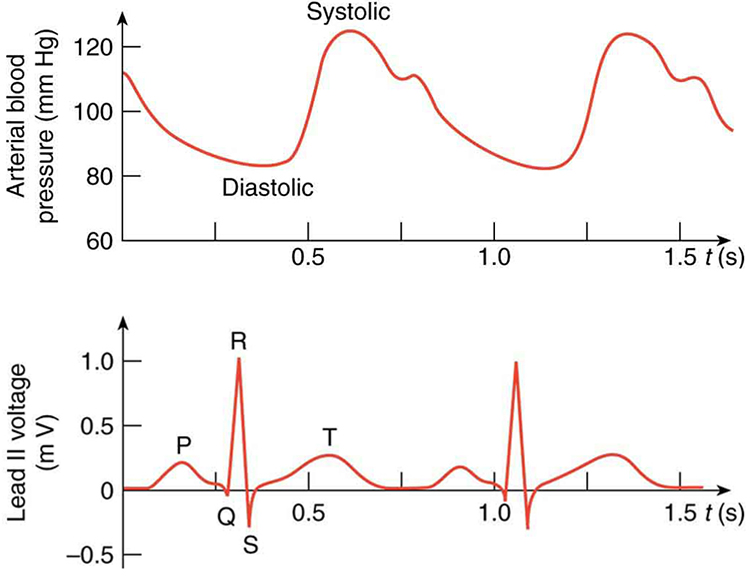
\includegraphics{ecg.jpeg}
\end{figure}


\subsubsection{Application or Uses }
\begin{itemize}
	\item
Taken together, the 12 leads of a state-of-the-art ECG can yield a wealth of information about the heart.
\item For example, regions of damaged heart tissue, called infarcts, reflect electrical waves and are apparent in one or more lead potentials.
\item Subtle changes due to slight or gradual damage to the heart are most readily detected by comparing a recent ECG to an older one. This is particularly the case since individual heart shape, size, and orientation can cause variations in ECGs from one individual to another.
\end{itemize}

\section{Artificial Pacemaker}
%\begin{tcolorbox}[title=Supplementary Information]
%\item



%\end{tcolorbox}
\subsubsection{Principle}
\begin{itemize}
%	\item The heart relies on electrical signals to maintain its rhythm. The movement of electrical signals causes the chambers of the heart to contract and relax.

%\item Also when a person has a heart attack, the movement of these electrical signals may be disturbed.
%\item An artificial pacemaker and a defibrillator can be used to initiate the rhythm of electrical signals.

\item The heart rate is normally controlled by electrical signals generated by the sino-atrial (SA) node, which is on the wall of the right atrium chamber.
\item This causes the muscles to contract and pump blood.
\item Sometimes the heart rhythm is abnormal and the heartbeat is too high or too low.

\item An aritificial pacemaker is an application of the RC timing circuit used to control heart rate.

\item The artificial pacemaker is inserted near the heart to provide electrical signals to the heart when needed with the appropriate time constant.

\item Pacemakers have sensors that detect body motion and breathing to increase the heart rate during exercise to meet the body’s increased needs for blood and oxygen.
\end{itemize}
\subsubsection{Uses}
\begin{itemize}
	\item Used to maintain normal heart beats in cases of heart block or arrhythmia.
	\item Electronic cardiac pacemaker may be temporary or permanent.
Temporary pacemakers are helpful to persons who have a transient
blockage of conduction pathway after a myocardial infraction or
cardiac surgery.
\item In cases of irreversible cardiac damage and complete conductive
pathway blockage a permanent pacemaker may be used.
\end{itemize}
\subsubsection{Procedural Details}
Refer to text. pg 173.

\section{Defibrillation}
\begin{itemize}
%	\item In a defibrillator, the delivery of a large charge in a short burst to a set of paddles across a person’s chest can be a lifesaver.
%\item The person’s heart attack might have arisen from the onset of fast, irregular beating of the heart—cardiac or ventricular fibrillation.
%\item  The application of a large shock of electrical energy can terminate the arrhythmia and allow the body’s pacemaker to resume normal patterns.

\item Defibrillator is an electric device used to deliver an electrical current (shock) of preset voltage to the heart through paddles placed on the chest wall (closed chest procedure).
\item
This current cause the entire
myocardium to depolarize completely at the moment of shock, thus
producing transient asystole and allowing the heart’s intrinsic
pacemaker to regain control.
\item The amount of energy required to produce
this effect is determined largely by the client’s transthoracic
impedance, or resistance to current flow.
\item Because of this factor, the
amount of energy that reaches the heart is less than the amount that
the defibrillator is charged to deliver.

\item The procedure is associated with potential hazards, particularly
myocardial damage.
\item The higher the amount of energy or frequency
of the shock, the greater the risk of injury.
\item  Advances in the equipments
now allow measurement of transthoracic impedance. Once impedance
is determined, the defibrillator automatically selects the amount of
current. It is expected this mode of defibrillation will reduce the risk
of complications.

\end{itemize}


\subsection{Automated External Defibrillator}
\begin{itemize}
	%Today it is common for ambulances to carry a defibrillator, which also uses an electrocardiogram to analyze the patient’s heartbeat pattern.  The device automatically diagnoses the patient’s heart condition and then applies the shock with appropriate energy and waveform.

	\item An automated external defibrillator or AED is a portable electronic
device that automatically diagnoses the potentially life threatening
cardiac arrhythmias of ventricular fibrillation and ventricular
tachycardia in a patient, and is able to treat them through defibrillation,
the application of electrical therapy which stops the arrhythmia,
allowing the heart to re-establish an effective rhythm.
\item  AEDs are
designed to be simple to use for the layman, and the use of AEDs
is taught in many first aid, first responder and basic life support (BLS)
level CPR classes. CPR is recommended in many cases before use of an AED.

\end{itemize}
\begin{figure}[H]
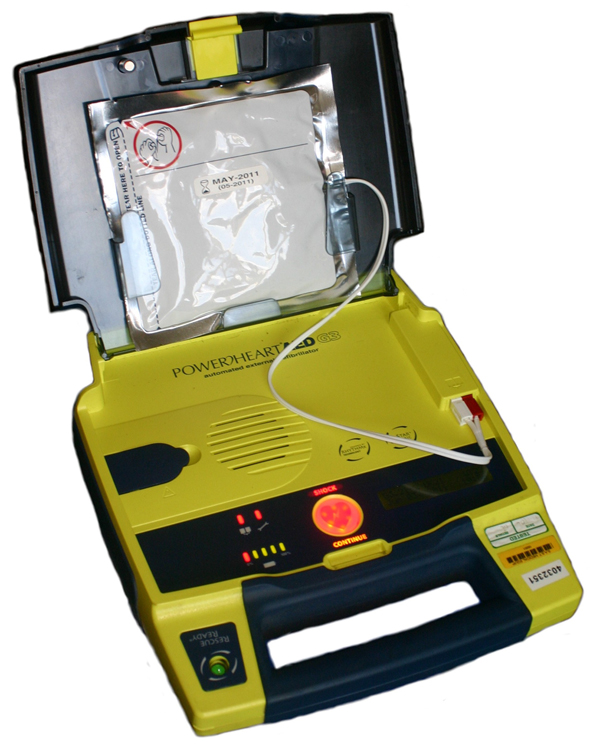
\includegraphics[scale=0.55]{aed.jpeg}
\centering
\caption{Automated external defibrillators are found in many public places. These portable units provide verbal instructions for use in the important first few minutes for a person suffering a cardiac attack.}
\end{figure}

\section{ECT}
Refer to text.

\chapter{X-rays}
\section{Basics}
\begin{itemize}
	\item X-rays are part of the electromagnetic spectrum.
	\item They are highly energetic radiation with a frequency beyond that of the UV spectrum.
	\item The first nobel prize in physics was awarded for the discovery of X-rays.
\end{itemize}

\subsection{Uses of X-rays}
\begin{itemize}
\item Dental and medical x rays that have become an essential part of medical diagnostics.
\item X rays are also used to inspect our luggage at airports,
\item They are also used for early detection of cracks in crucial aircraft components.
\end{itemize}


\section{CT Scan}
\begin{figure}[h]
%\end{figure}
%\begin{figure}
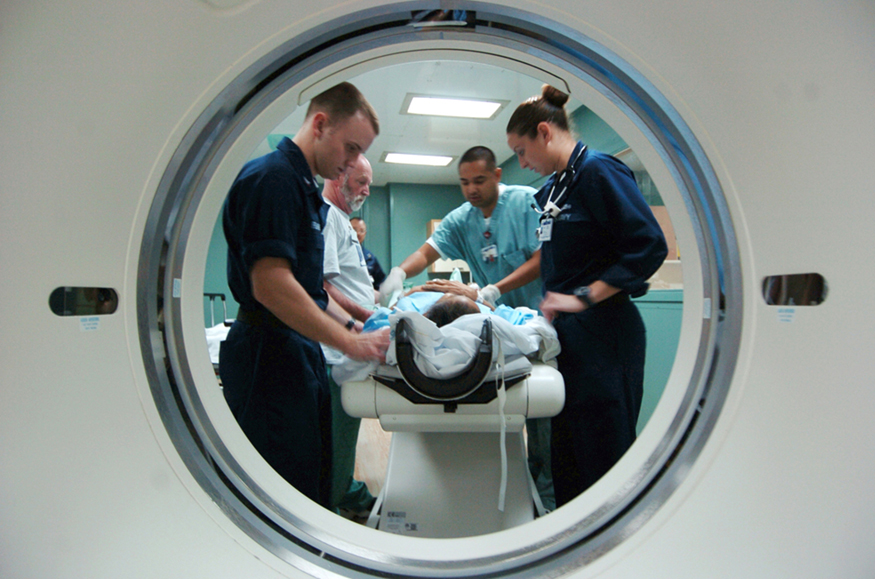
\includegraphics[scale=0.53]{ct-mach}
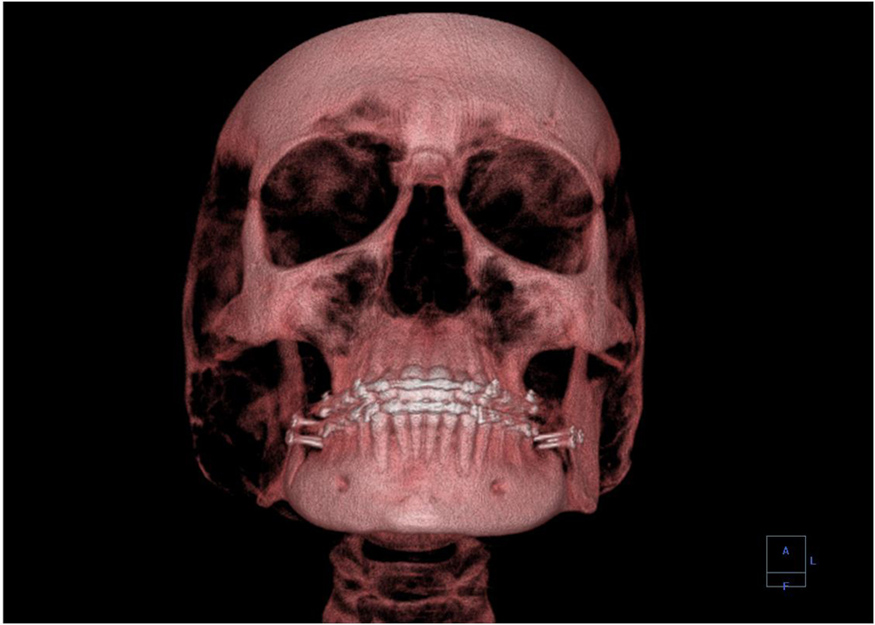
\includegraphics[scale=0.49]{ct-scan}
\caption{On the left, a patient being positioned into a CT scanner.
On  the right, the 3D image of a skull produced by CT.}
\end{figure}
\subsection{Principle}
\begin{itemize}
\item A standard x ray gives only a two-dimensional view of the object.
\item Dense bones might hide images of soft tissue or organs.
\item If you took another x ray from the side of the person (the first one being from the front), you would gain additional information.
\item While shadow images are sufficient in many applications, far more sophisticated images can be produced with modern technology.
\end{itemize}
\subsection{Process}
\begin{itemize}
	\item X rays are passed through a narrow section (called a slice) of the patient’s body (or body part) over a range of directions.
	\item An array of many detectors on the other side of the patient registers the x rays.
	\item The system is then rotated around the patient and another image is taken, and so on.
	\item The x-ray tube and detector array are mechanically attached and so rotate together.
	\item Complex computer image processing of the relative absorption of the x rays along different directions produces a highly-detailed image.
	\item Different slices are taken as the patient moves through the scanner on a table.
	\item Multiple images of different slices can also be computer analyzed to produce three-dimensional information, sometimes enhancing specific types of tissue,
\end{itemize}
\subsection{Uses}
Refer. to \url{https://www.radiologyinfo.org/en/info.cfm?pg=bodyct}

\chapter{MRI}
\section{Basics}
\begin{itemize}
\item Magnetic resonance imaging (MRI) is one of the most useful and rapidly growing medical imaging tools.
\item It non-invasively produces two-dimensional and three-dimensional images of the body that provide important medical information
\item It has none of the hazards like those associated with x-rays.
\item  MRI is based on an effect called nuclear magnetic resonance (NMR)
\end{itemize}
\section{Mechanism of Operation}
Refer to text.

\section{Uses}
\begin{itemize}
\item The location and density of protons give a variety of medically useful information, such as organ function, the condition of tissue (as in the brain), and the shape of structures, such as vertebral disks and knee-joint surfaces.
\item MRI can also be used to follow the movement of certain ions across membranes, yielding information on active transport, osmosis, dialysis, and other phenomena.
\item With excellent spatial resolution, MRI can provide information about tumors, strokes, shoulder injuries, infections, etc.
\end{itemize}
\section{Disadavantages}
\begin{itemize}
\item While MRI images are superior to x rays for certain types of tissue and have none of the hazards of x rays, they do not completely supplant x-ray images.

\item MRI is less effective than x rays for detecting breaks in bone, for example, and in imaging breast tissue, so the two diagnostic tools complement each other.
\item MRI images are also expensive compared to simple x-ray images and tend to be used most often where they supply information not readily obtained from x rays.

\item Another disadvantage of MRI is that the patient is totally enclosed with detectors close to the body for about 30 minutes or more, leading to claustrophobia.
\item It is also difficult for the obese patient to be in the magnet tunnel.

%Over the last decade, the development of much faster scans, called “functional MRI” (fMRI), has allowed us to map the functioning of various regions in the brain responsible for thought and motor control. This technique measures the change in blood flow for activities (thought, experiences, action) in the brain. The nerve cells increase their consumption of oxygen when active. Blood hemoglobin releases oxygen to active nerve cells and has somewhat different magnetic properties when oxygenated than when deoxygenated. With MRI, we can measure this and detect a blood oxygen-dependent signal. Most of the brain scans today use fMRI.
\end{itemize}
\end{document}
